\hypertarget{an-introduction-to-scrum}{%
\section{An Introduction to Scrum}\label{an-introduction-to-scrum}}

\begin{itemize}
\tightlist
\item
  Scrum is an agile process that allows us to \textbf{focus on
  delivering the highest business value} in the shortest time.
\item
  It allows us to rapidly and \textbf{repeatedly inspect actual working
  software} (every two weeks to one month).
\item
  The business sets the priorities. Teams self-organize to determine the
  best way to \textbf{deliver the highest priority features}.
\end{itemize}




\hypertarget{Principles}{%
\subsection{Principles}\label{Principles}}
\begin{figure}[H]
\centering
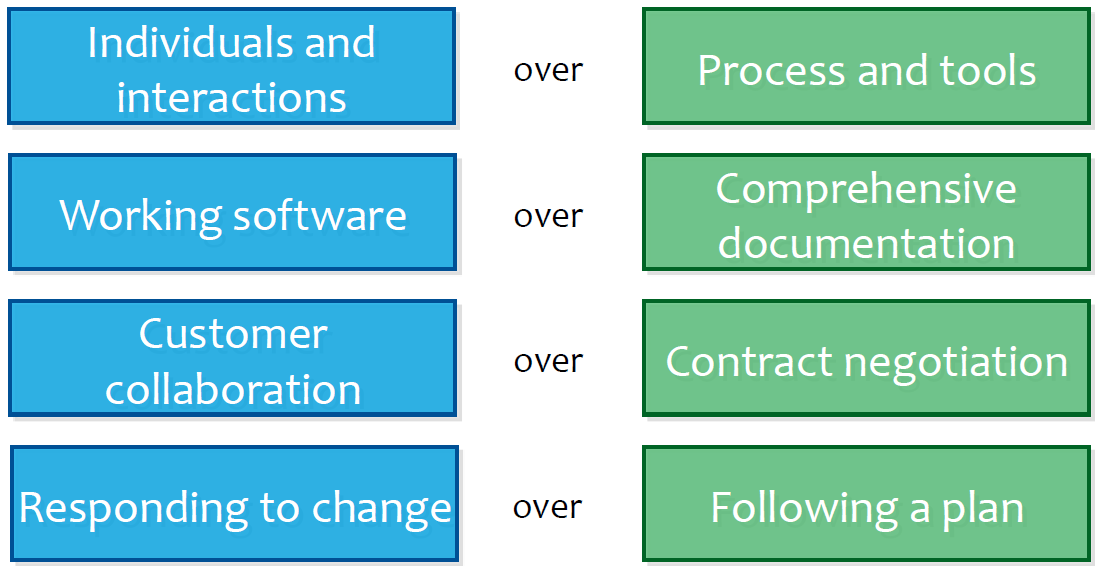
\includegraphics[width=0.5\textwidth]{figures/ScrumPrinciples.png}
\caption{Scrum Principles}
\end{figure}






\hypertarget{characteristics}{%
\subsection{Characteristics}\label{characteristics}}

\begin{itemize}
\tightlist
\item
  Self-organizing teams

  \begin{itemize}
  \tightlist
  \item
    There is no project leader
  \item
    Every team-member is on the same level in the hirarchy
  \end{itemize}
\item
  Product progresses in a series of month-long ``sprints''
\item
  Requirements are captured as items in a list of ``product backlog''

  \begin{itemize}
  \tightlist
  \item
    User stories
  \end{itemize}
\item
  No specific engineering practices prescribed
\item
  Uses generative rules to create an agile environment for delivering
  projects
\item
  One of the ``agile processes''
\end{itemize}

\hypertarget{components}{%
\subsection{Components}\label{components}}

\begin{figure}[H]
\centering
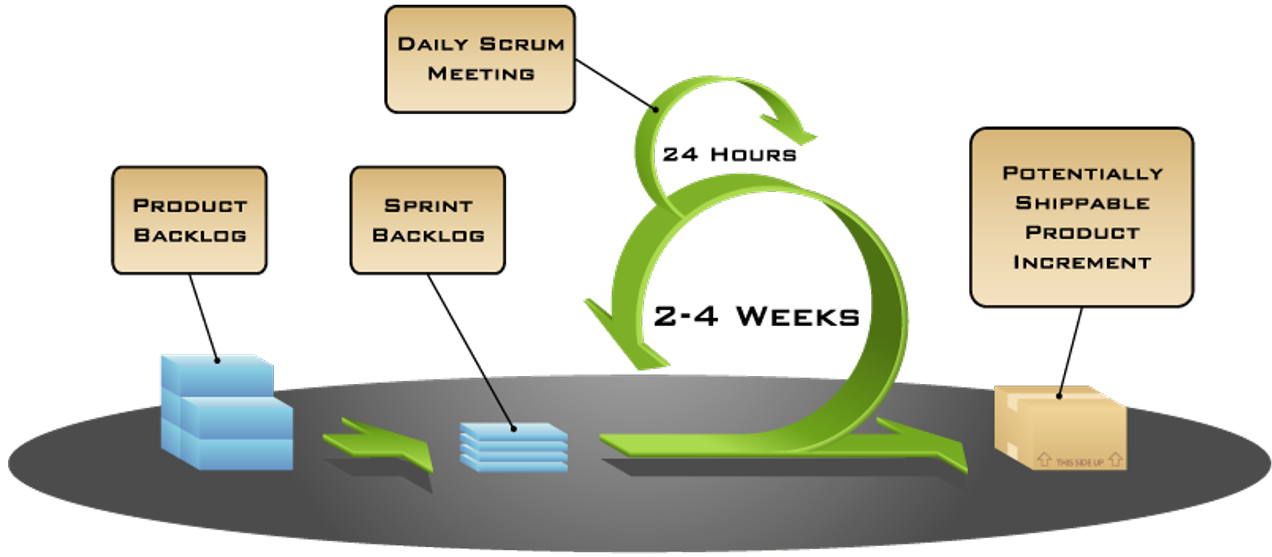
\includegraphics[width=0.5\textwidth]{figures/scrumComponents.png}
\caption{Scrum Components}
\end{figure}


\hypertarget{product-backlog}{%
\subsubsection{Product backlog}\label{product-backlog}}

\begin{itemize}
\tightlist
\item
  All requirements
\item
  Prioritized by the product owner
\item
  Ideally expressed such that each item has value to the user or
  customers of the product
  
  \item 
  The priority can change every sprint
\end{itemize}

\hypertarget{advantage}{%
\paragraph{Advantage}\label{advantage}}

\begin{itemize}
\tightlist
\item
  Compared to the system specification (Pflichtenhef) you are able to
  adjust your requirements during the project.
\item
  If you have to do a full system specification at the start of a
  project, this costs a lot of time and you propably forget something
\end{itemize}

\hypertarget{disadvantage}{%
\paragraph{Disadvantage}\label{disadvantage}}
\begin{itemize}
\tightlist
\item
    No complete overview on the whole project 
\item
    High communication and coordination overhead
\item
    No concrete recommondations how to act
\item
    Insecurities due to absence of hierarchies or responsibilities
\end{itemize}

\hypertarget{ingredients}{%
\subsection{Ingredients}\label{ingredients}}

\hypertarget{no-interruption}{%
\subsubsection{No interruption}\label{no-interruption}}

The developers must not be interrupted during a sprint.

\hypertarget{roles}{%
\subsubsection{Roles}\label{roles}}

\begin{itemize}
\tightlist
\item
  Product owner

  \begin{itemize}
  \tightlist
  \item
    \textbf{Define} the features of the product
  \item
    \textbf{Decide} on release date and content
  \item
    Be responsible for the profitability of the product (ROI)
  \item
    \textbf{Prioritize features} according to market value
  \item
    Adjust features and priority every iteration, as needed
  \item
    Accept or reject work results
  \end{itemize}
\item
  Scrum master

  \begin{itemize}
  \tightlist
  \item
    Responsible for enacting Scrum values and practices
  \item
    Removes impediments (Hindernisse)
  \item
    Ensure that the team is fully functional and productive
  \item
    Enable close cooperation across all roles and functions
  \item
    Shield the team from external interferences
    \item
    Helps that the team learns from experience
  \end{itemize}
  
\item
  Team
  \begin{itemize}
  \tightlist
  \item
    Typically 5-9 people
  \item
    Cross-functional:

    \begin{itemize}
    \tightlist
    \item
      Programmers, testers, user experience designers, etc.
    \end{itemize}
  \item
    Members should be full-time
  \item
    Teams are self-organizing
  \item
    Membership should change only between sprints
  \end{itemize}
\end{itemize}

























\hypertarget{ceremonies}{%
\subsubsection{Ceremonies}\label{ceremonies}}

\begin{itemize}
\tightlist
\item
  Sprint planning

  \begin{itemize}
  \tightlist
  \item
    Sprint prioritization

    \begin{itemize}
    \tightlist
    \item
      Analyze and evaluate product backlog
    \item
      Select sprint goal

      \begin{figure}[H]
\centering
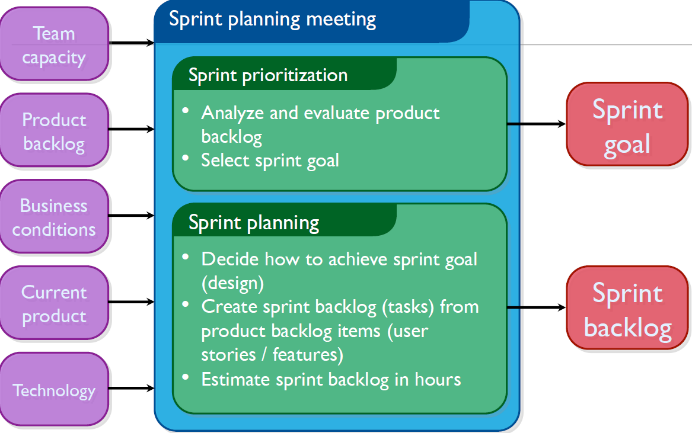
\includegraphics[width=0.5\textwidth]{figures/ScrumCeremonies.png}
\caption{Sprint Planning}
\end{figure}
    \end{itemize}
  \item
    sprint planning

    \begin{itemize}
    \tightlist
    \item
      Decide how to achieve sprint goal (design)
    \item
      Create sprint backlog (tasks) from product backlog items (user
      stories / features)
    \item
      Estimate sprint backlog in hours
    \end{itemize}
  \end{itemize}
\item
  Sprint review

  \begin{itemize}
  \tightlist
  \item
    Team presents what it accomplished during the sprint
  \item
    Typically takes the form of a demo of new features or underlying
    architecture
  \item
    Informal (2 hour prep time rule, no slides)
  \end{itemize}
\item
  Sprint retrospective

  \begin{itemize}
  \tightlist
  \item
    Periodically take a look at what is and is not working
  \item
    Done after every sprint
    \item 
    Duration should not exceed 30 min
    \item 
    Everyone participates (Scrum Master, Product Owner etc.). Everyone shares their opinion to certain work what they like or dislike.
  \end{itemize}
\item
  Daily scrum meeting

  \begin{itemize}
  \tightlist
  \item
    Daily, 15 Minutes, Stand-up
  \item
    What did you do yesterday?
  \item
    What will you do today?
  \item
    Where are your problems?
  \end{itemize}
\end{itemize}

\hypertarget{artifacts}{%
\subsubsection{Artifacts}\label{artifacts}}

\begin{itemize}
\tightlist
\item
  Products backlog
\item
  Sprint backlog
\item
  Burndown charts
  \begin{itemize}
      \item To far right, remove items from backlog
      \item To far left, add items from backlog
      \item Scrum Master should have a check if first prio is done first!
  \end{itemize}
\end{itemize}

\hypertarget{scrum-board}{%
\subsubsection{Scrum Board}\label{scrum-board}}



\begin{figure}[H]
\centering
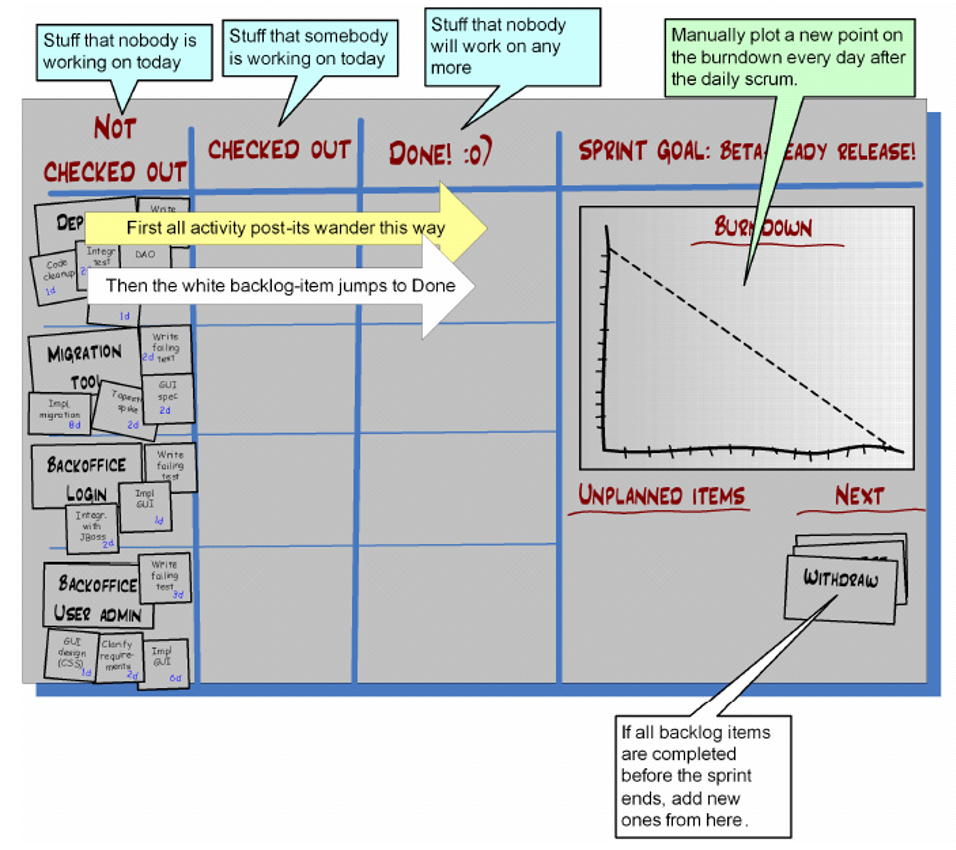
\includegraphics[width=0.5\textwidth]{figures/scrumBoard.png}
\caption{Scrum Board}
\end{figure}

\hypertarget{some-warnings-from-the-scrum-board}{%
\paragraph{Some warnings from the scrum
board}\label{some-warnings-from-the-scrum-board}}

\begin{figure}[H]
\centering
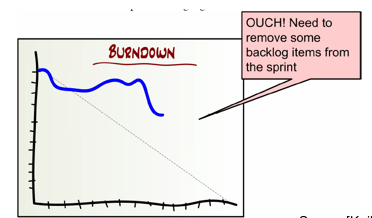
\includegraphics[width=0.5\textwidth]{figures/burndownAlert.png}
\caption{Burndown Alerts}
\end{figure}

\begin{itemize}
\tightlist
\item
  This indicates, that the team is too slow
\item
  It is also possible that the burndown is falling too fast. Then you
  have to add some items to the current sprint
\end{itemize}

\begin{figure}[H]
\centering
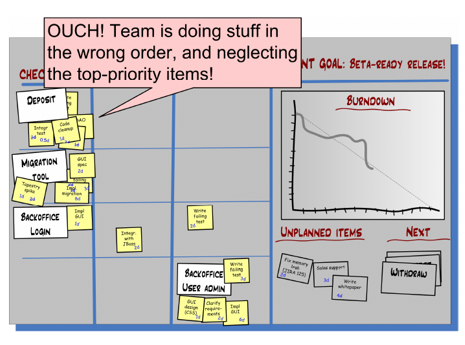
\includegraphics[width=0.5\textwidth]{figures/wrongPrio.png}
\caption{Wrong Prio}
\end{figure}

\begin{figure}[H]
\centering
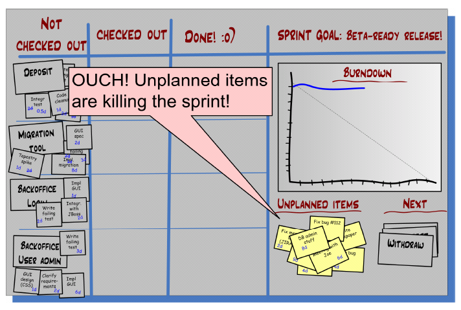
\includegraphics[width=0.5\textwidth]{figures/unplannedAlert.png}
\caption{Unplanned Items Alert}
\end{figure}




\clearpage